\scanpage{14}
% archive foliation: 13
Soit $X\in C$, avec un groupe $\unsure{\Gamma|G}$ d'automorphismes \inserted{à droite}. On suppose que pour $\forall$ sous-groupe $H$ de $G$, \deleted{et $\forall$ \illegible{1}} $X/H$ existe, et que pour $H'\subset H$ \inserted{invariant} d'indice fini $r$ dans $H$, \deleted{$X/H'\longrightarrow X/H$ soit dans $(\mathcal N)$ et de degré $r$. (on a encore des exemples, et des \illegible{2}, pour les)} \unsure{l'objet|le couple} $X/H'$ avec groupe à opérateurs fini $H/H'$ soit \uline{non ramifié}, et $X/H'\longrightarrow X/H=(X/H')/(H/H')$ est $\in(\mathcal N)$. Soit $C'$ la catégorie des ensembles $E$ où $\Gamma$ opère, et pour $E/\Gamma$ soit fini. Alors \deleted{\unsure{pour}} pour $\forall\ E\in C'$, $X\times_{(\Gamma)}E$ \uline{existe}, soit $\Phi(E)=X\times_{(\Gamma)}E$,

\margin{\uuline{\unsure{à développer}}}
\figure{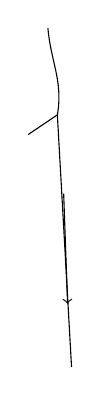
\begin{tikzpicture}\draw (0,0) to[out=-85,in=80] (0.12,-1.1)--(0.3,-4.3);\draw (0.12,-1.1)--(-0.25,-1.35);\draw[->] (0.2,-2.1)--(0.25,-3.5);\end{tikzpicture}}
$\Phi$ est donc un foncteur $\unsure{C'|E'}\longrightarrow C$, commutant aux sommes finies, et on sait de plus que $\Phi$ transforme morphisme de degré $r$ en morphisme de degré $r$ (\unsure{id : fait aussi sur} $\mathcal N$). De plus, il transforme \deleted{morphismes} \inserted{conserve} les \unsure{compos}\ldots
